\chapter{Community Composition Measures}

%% ============================================
%% PC vs Pollution Score Regression Results
%% ============================================

\begin{table}[htbp]
    \centering
    \caption{Significant Species PC vs Pollution Score Regressions}
    \label{tab:04_pc_pollution_regression}
    \small
    \begin{tabular}{cclccccc}
        \toprule
        \textbf{Cluster} & \textbf{PC} & \textbf{Var.(\%)} & \textbf{$R^2$} & \textbf{$\bar{R}^2$} & \textbf{Coef.} & \textbf{$t$-stat} & \textbf{$n$} \\
        \midrule
        0 & PC2 & 13.42 & 0.4223 & 0.4016 & $-0.0594$ & $-4.524^{***}$ & 30 \\
        2 & PC1 & 35.16 & 0.5039 & 0.4625 & $-0.0907$ & $-3.491^{**}$ & 14 \\
        \bottomrule
    \end{tabular}
    
    \vspace{0.5em}
    \footnotesize
    \textit{Note:} Only significant regressions shown ($p < 0.01$).
    Significance: $^{**}p < 0.01$; $^{***}p < 0.001$
\end{table}

%% ============================================
%% Pollution PC vs Species PC Regression Results
%% ============================================

\begin{table}[htbp]
    \centering
    \caption{Significant Pollution PC vs Species PC Regressions ($p < 0.05$)}
    \label{tab:04_pollution_pc_species_pc}
    \small
    \begin{tabular}{ccccccc}
        \toprule
        \textbf{Cluster} & \textbf{Poll. PC} & \textbf{Spec. PC} & \textbf{Var.(\%)} & \textbf{$R^2$} & \textbf{Slope} & \textbf{$n$} \\
        \midrule
        2 & PC2 & PC1 & 35.16 & 0.4321 & $-0.151^{*}$ & 14 \\
        0 & PC3 & PC2 & 13.42 & 0.2800 & $-0.159^{**}$ & 30 \\
        0 & PC4 & PC5 & 8.46 & 0.2600 & $-0.097^{**}$ & 30 \\
        0 & PC2 & PC2 & 13.42 & 0.2063 & $-0.096^{*}$ & 30 \\
        0 & PC2 & PC4 & 9.81 & 0.1594 & $0.072^{*}$ & 30 \\
        1 & PC2 & PC1 & 19.35 & 0.1172 & $0.085^{**}$ & 60 \\
        1 & PC1 & PC2 & 15.06 & 0.1025 & $-0.057^{*}$ & 60 \\
        1 & PC2 & PC6 & 6.40 & 0.0803 & $-0.041^{*}$ & 60 \\
        \bottomrule
    \end{tabular}
    
    \vspace{0.5em}
    \footnotesize
    \textit{Note:} Var.(\%) = variance explained by the Species PC. \\
    \textit{Poll. PC = Pollution Principal Component; Spec. PC = Species Principal Component.} \\
    \textit{Significance: $^{*}p < 0.05$; $^{**}p < 0.01$}
    \end{table}



% \begin{figure}[htbp]
%     \centering
%     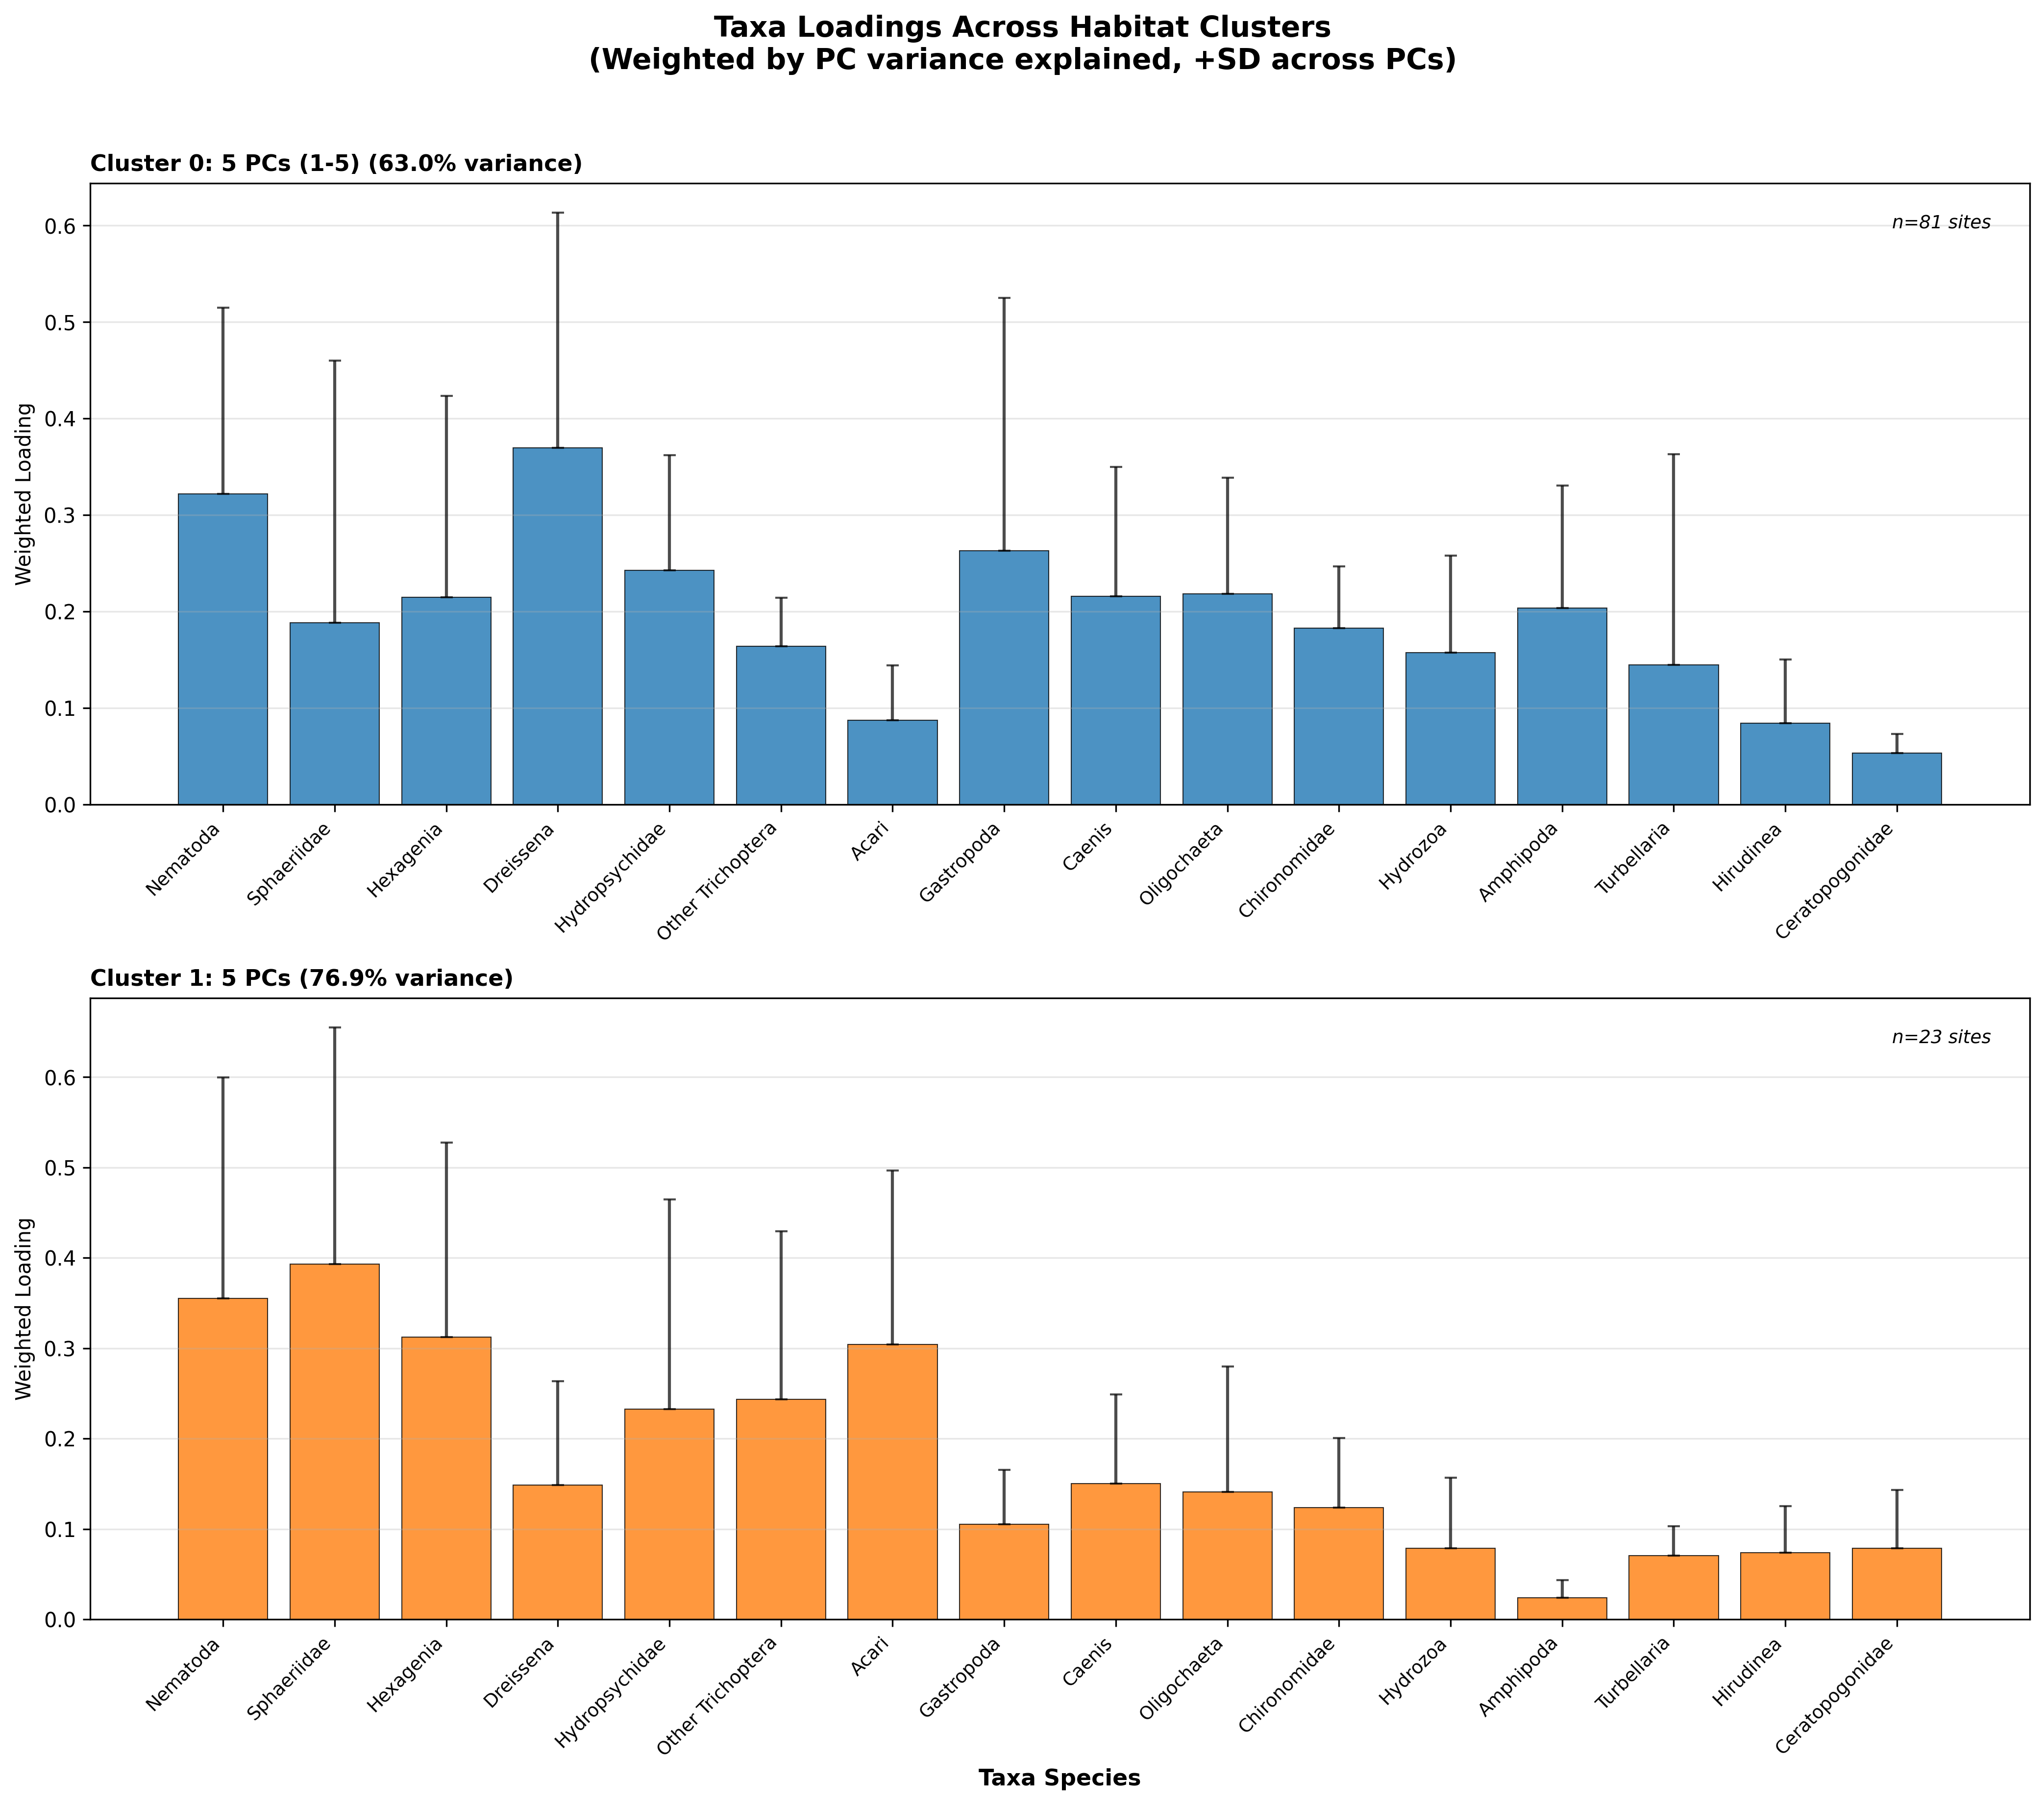
\includegraphics[width=0.9\textwidth]{../results/figures/04_community_composition_measures/figure1_taxa_loadings.png}
%     \caption{Taxa Loadings}
%     \label{fig:04_taxa_loadings}
% \end{figure}

\begin{figure}[htbp]
    \centering
    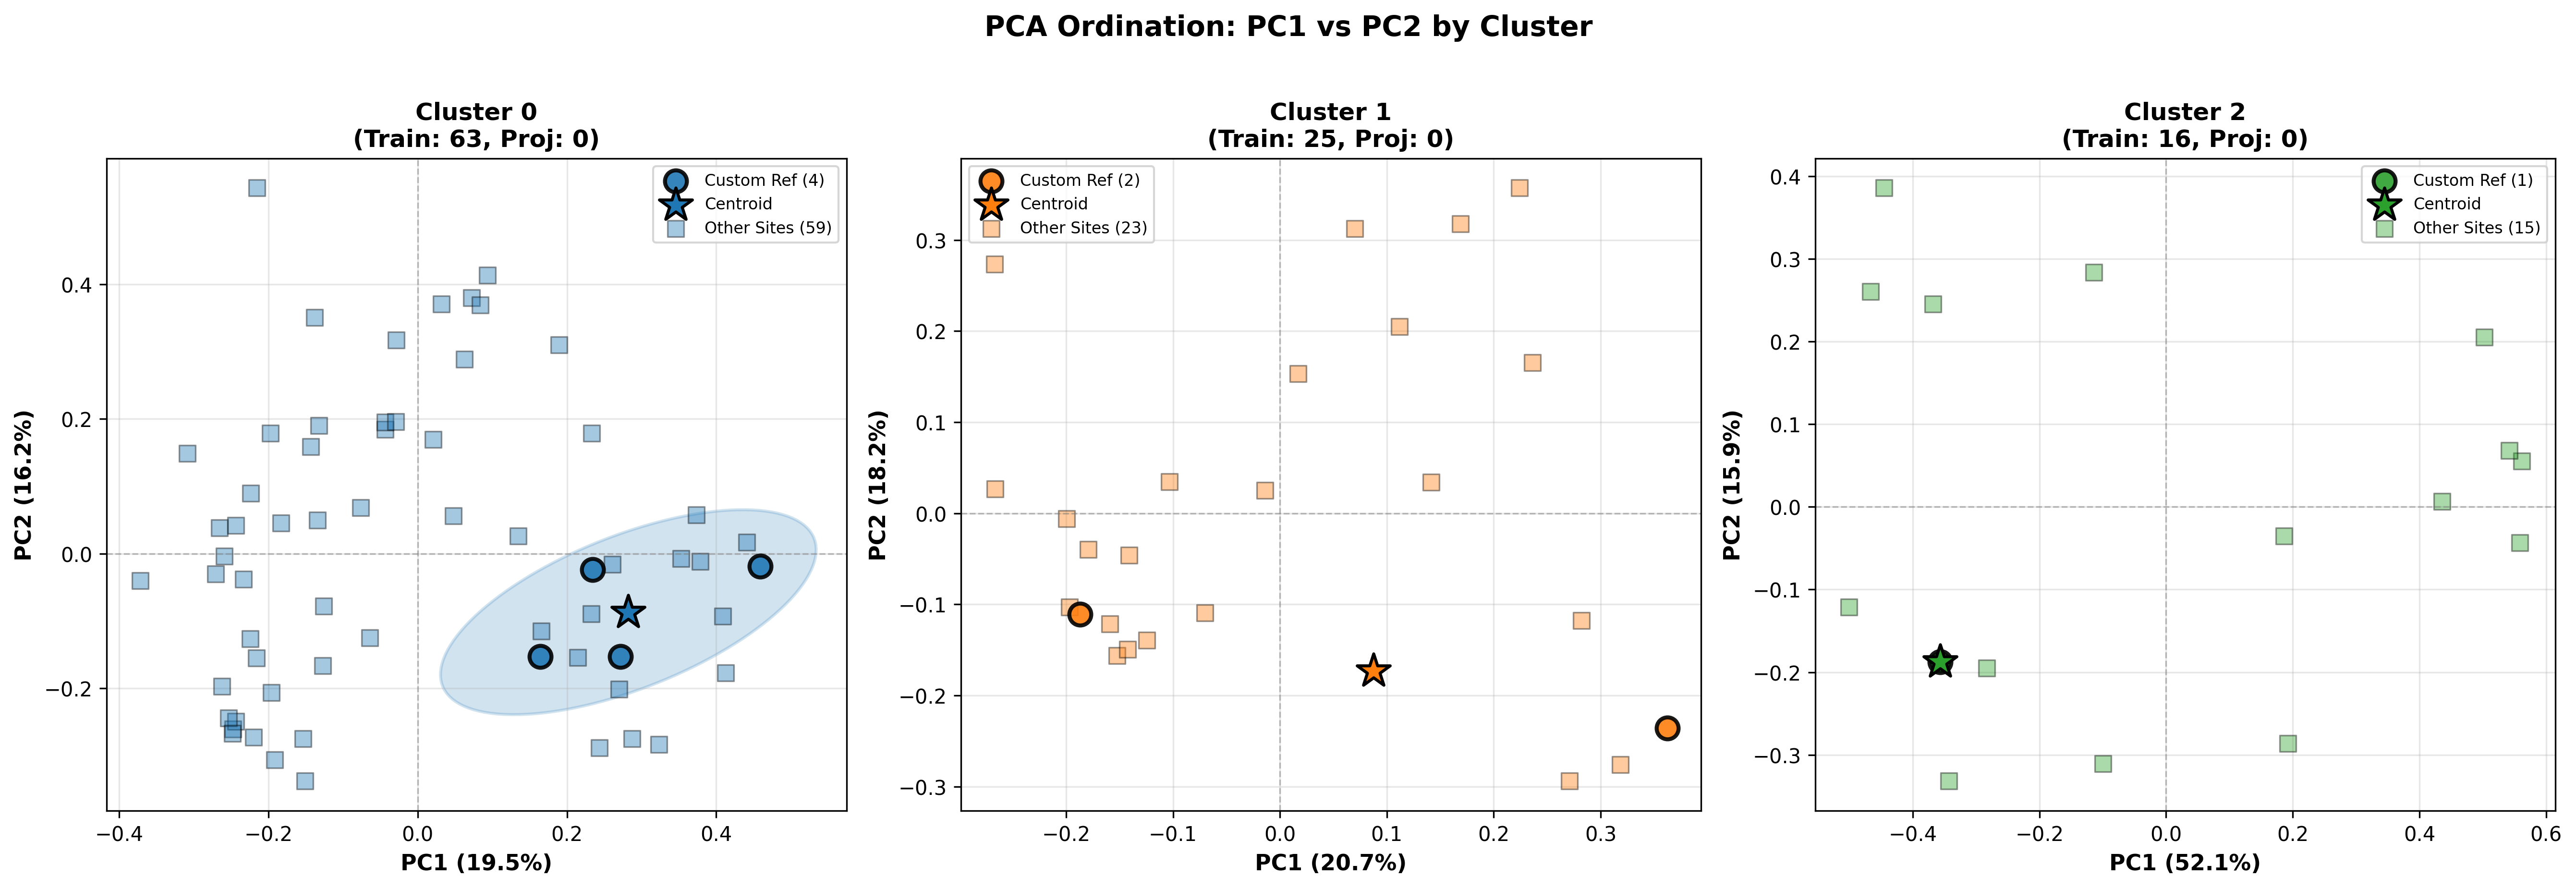
\includegraphics[width=0.9\textwidth]{../results/figures/04_community_composition_measures/figure2_ordination.png}
    \caption{Ordination}
    \label{fig:04_ordination}
\end{figure}

\begin{figure}[htbp]
    \centering
    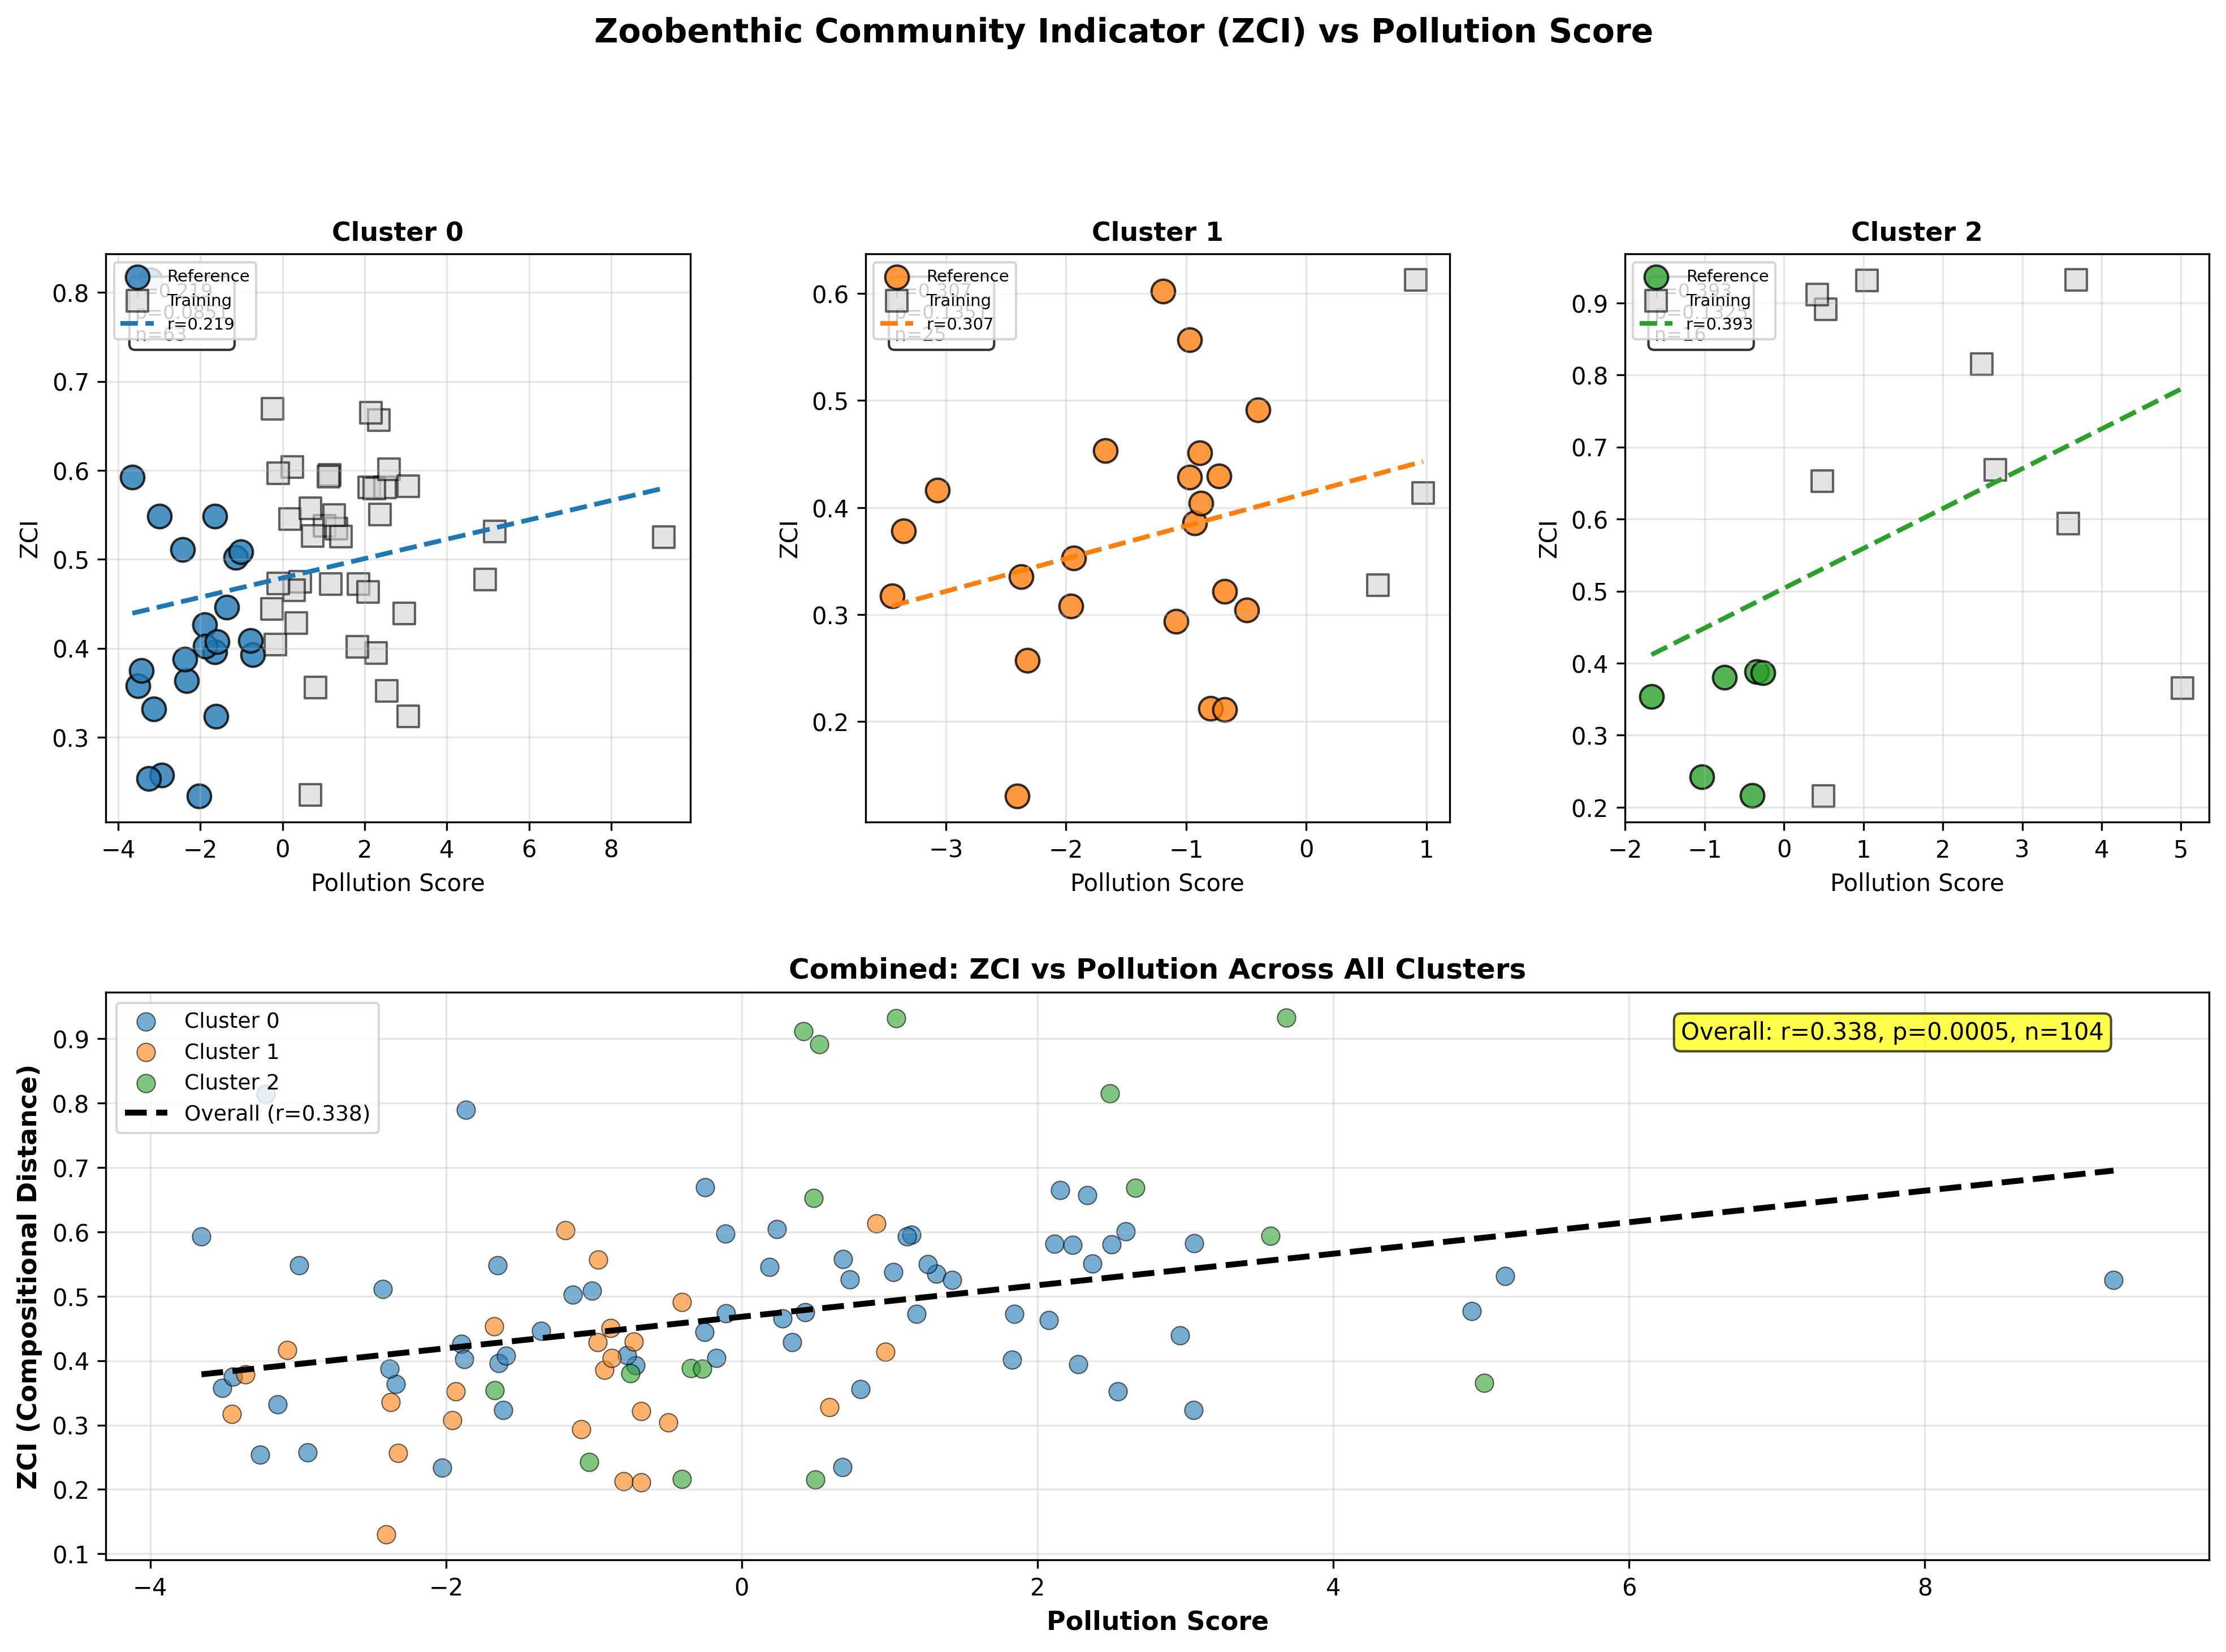
\includegraphics[width=0.9\textwidth]{../results/figures/04_community_composition_measures/figure3_zci_vs_pollution.png}
    \caption{ZCI vs Pollution}
    \label{fig:04_zci_vs_pollution}
\end{figure}

\begin{figure}[htbp]
    \centering
    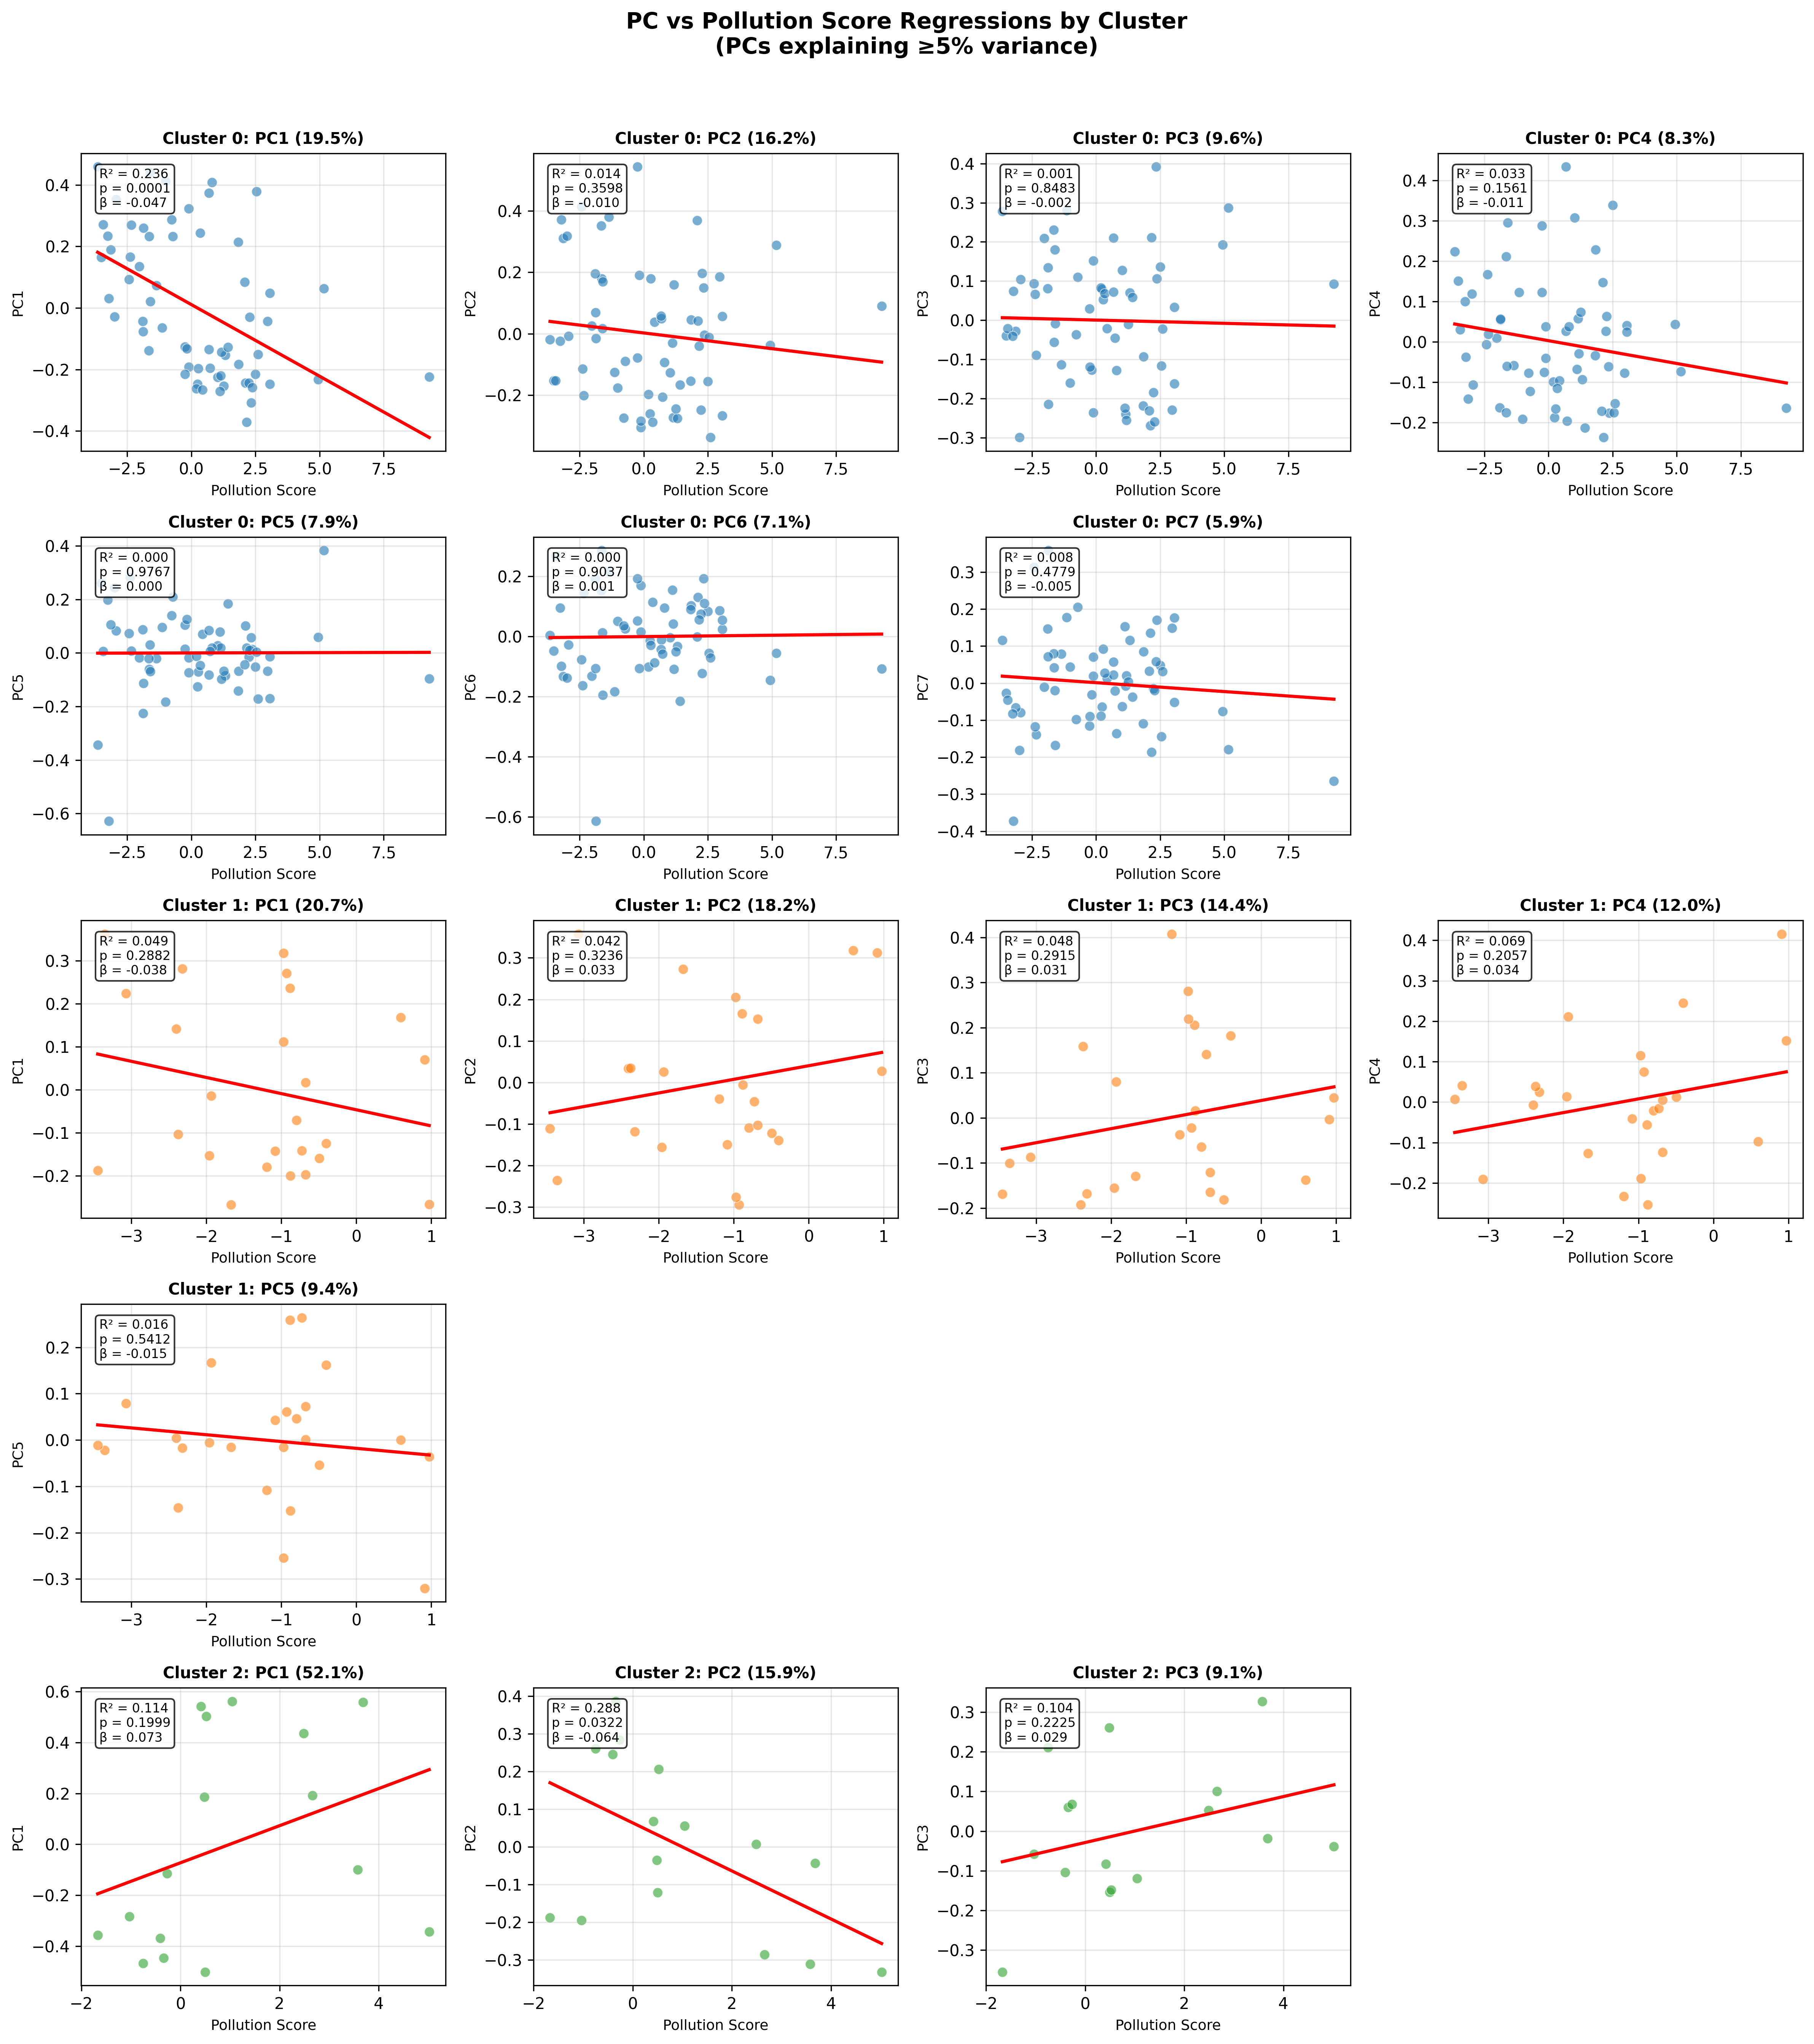
\includegraphics[width=0.9\textwidth]{../results/figures/04_community_composition_measures/figure4_pc_regression.png}
    \caption{PC Regression}
    \label{fig:04_pc_regression}
\end{figure}

\begin{figure}[htbp]
    \centering
    \includegraphics[width=0.9\textwidth]{../results/figures/04_community_composition_measures/figure5_pollution_vs_species_pc.png}
    \caption{Pollution vs Species PC}
    \label{fig:04_pollution_vs_species_pc}
\end{figure}
